\section{Processing}

Overview text required.





\subsection{Image Acquisition Pipeline}

\begin{center}
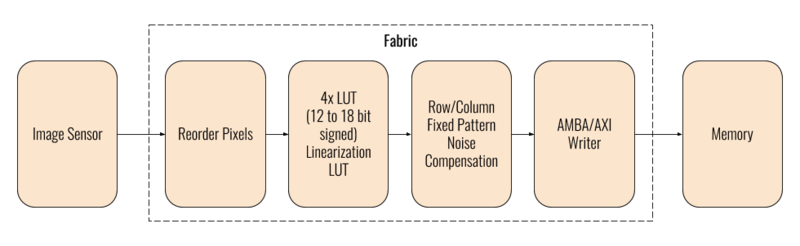
\includegraphics[height=5cm]{images/800px-AXIOM_Beta_Image_Acquisition_Pipeline}
\end{center}





\subsection{HDMI Image Processing/Output Pipeline}

\begin{center}
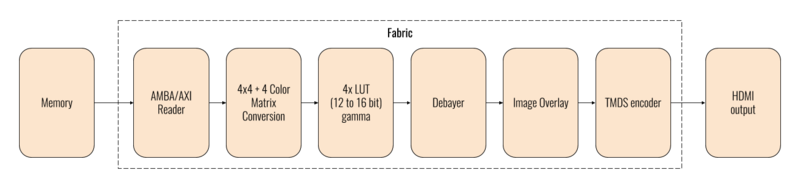
\includegraphics[height=4cm]{images/800px-AXIOM_Beta_HDMI_Image_Processing_Pipeline}
\end{center}





\subsection{SDI Image Processing/Output Pipeline}


ToDo - ETA Dec 2017.





\subsection{Image Processing Nodes}

\textbf{Debayering}\\

A planned feature is to generate this FPGA code block with "dynamic reconfiguration" meaning that the actual debayering algorithm can be replaced at any time by loading a new FPGA binary block at run-time. This tries to simplify creating custom debayering algorithms with a script like programming language that can be translated to FPGA code and loaded into the FPGA dynamically for testing. 

\textbf{Peaking}\\

Peaking marks high image frequency areas with colored dot overlays. These marked areas are typically the ones "in-focus" currently so this is a handy tool to see where the focus lies with screens that have lower resolution than the camera is capturing.\\

\textbf{Handy Custom Parameters:}\\

- color\\
- frequency threshold \\


\textbf{Potential Problems:}\\

There are sharper and softer lenses so the threshold depends on the glass currently used. For a sharp lens the peaking could show areas as "in-focus" if they actually aren't and for softer lenses the peaking might never show up at all because the threshold is never reached.\\